\label{chapter:related_work}

With the advancements driven by successful architectures like GATs and GCNs, analyzing and learning from graph data has become a more popular topic. GNNs have become a standard toolkit in the field and new ideas are developed in an increasing pace. In an attempt to increase comparability between architectures, \cite{dwivedi2020benchmarking} proposes a new benchmarking framework and point out flaws in common practices. The question how to fairly evaluate GNN architectures is a complicated one and outside the scope of this report. However, we'll focus on data sets and pass some criticism on evaluation methods used in the orginal GAT paper.

To begin with, data sets used for transductive tasks, namely Cora and Citeseer, are not large enough. According to the authors, small scale data sets "can become a liability in the long run as new GNN models will be designed to overfit the small test sets instead of searching for more generalizable architectures". As a result of this, all GNNs considered in the paper performed almost statistically the same on them. To find differences in performance, one should consider larger datasets. It is worth noting that \cite{velickovic2018graph} included the Pubmed dataset as well, which includes about 20k nodes and would still be considered small-scale. All "medium-scale" data sets proposed by the authors contain mutliple graphs with more than a million nodes total, except for a single social network graph with about 236k nodes.

Additionally, models should be evaluated on different tasks.  The authors presented 7 datasets to account for the variability of machine learning tasks on graphs. When compared to other models, GAT often performs slightly worse than state-of-the-art competitors, but manages to deliver the best results within the class of GCNs. However, some previously considered inferior architectures like MoNet outmatch GATs when compared on the right dataset. Comparisons for node classification on the PATTERN dataset shows a 10 percent accuracy advantage of MoNet over GAT, see Figure \ref{fig:gat_benchmark}.


Still, the authors conclude that GCN models\footnote{With the development of more diverse architectures, message-parsing GNNs based on neighborhood aggregation have been considered a \textit{class} of models, labeled GCNs. Among others, this includes GAT, MoNet and the vanilla GCN proposed by \cite{kipf2017semisupervised}.} like GAT outperform more recent GNNs which were designed to better distinguish between graph structures. Additionally, models that assign different importance to neighbors in the aggregation step like GAT yielded the best results. Given these promising results, they argue that analyzing the expressivity of attention mechanisms would be a good subject for future research.

\begin{figure}[h]
    \centering
    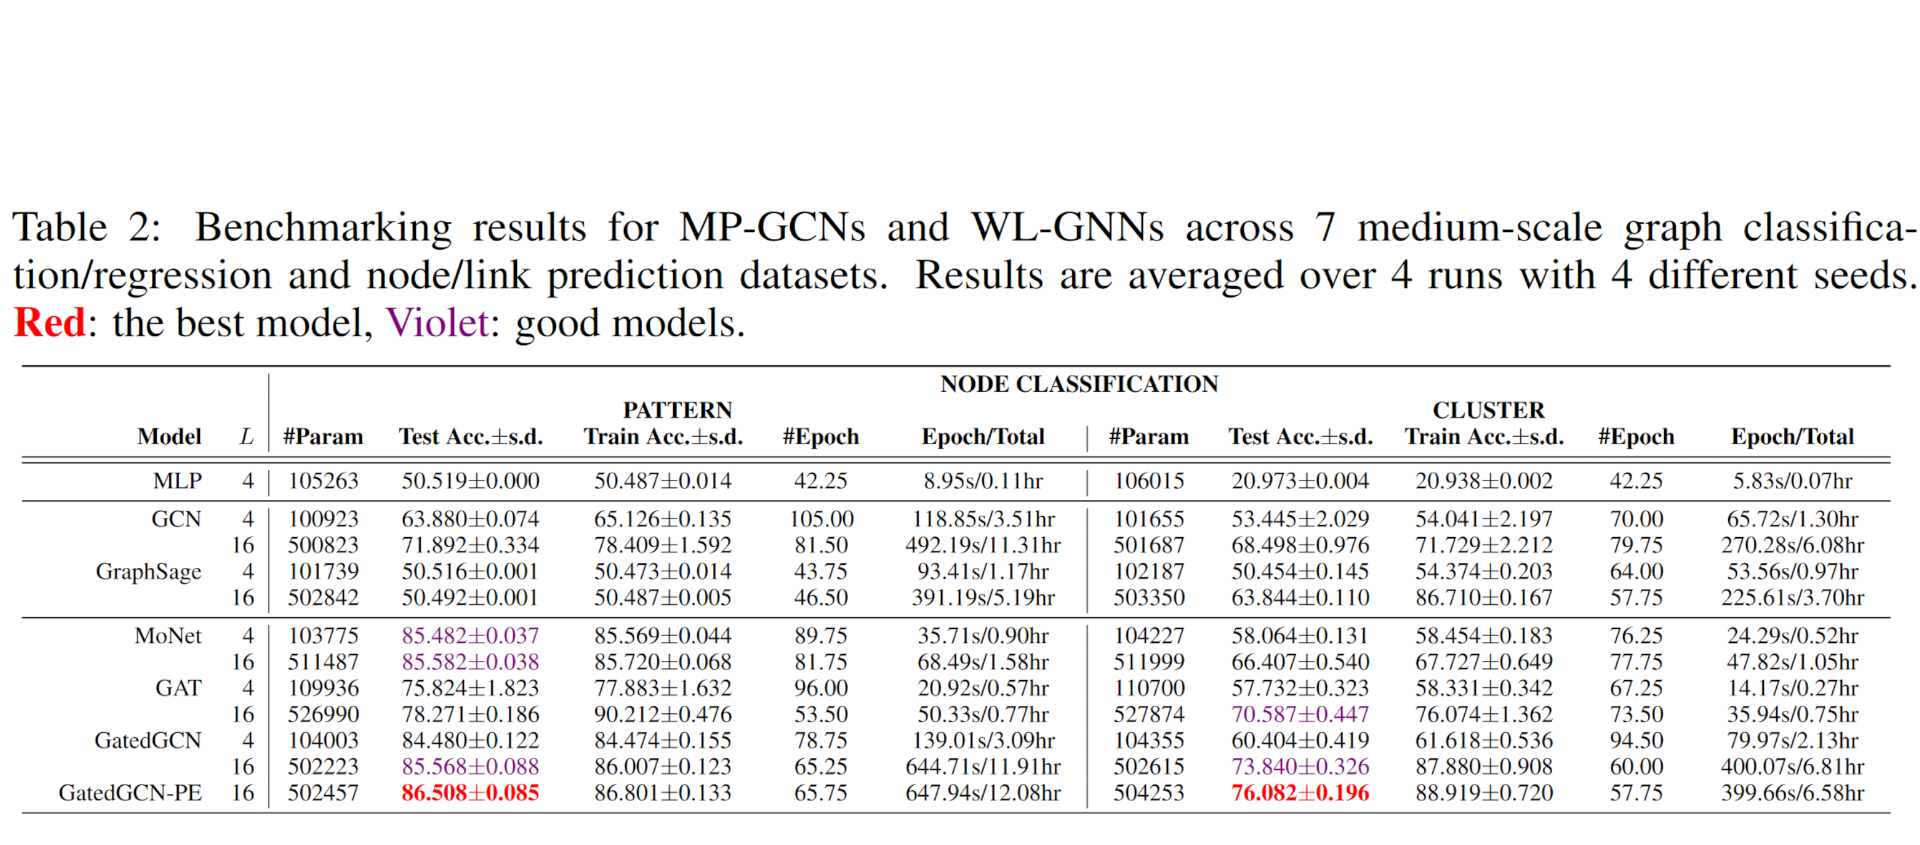
\includegraphics[width=0.99\textwidth]{img/benchmark_gat_worse.PNG}
    \caption{GAT performs worse than MoNet on specific tasks. \cite{dwivedi2020benchmarking}}
    \label{fig:gat_benchmark}
\end{figure}